\documentclass[14pt, aspectratio=169, handout]{beamer}
\usetheme{Copenhagen}
\usecolortheme{seahorse}
\setbeamertemplate{navigation symbols}{}
\setbeamertemplate{headline}{}

%\usepackage{pgfpages}
%\pgfpagesuselayout{4 on 1}[a4paper, border shrink=5mm]

\usepackage{graphicx} % Required for inserting images
\usepackage{multicol}
%\usepackage{enumitem}
\usepackage{amsfonts}
\usepackage{amsmath}

\title{SST1 Übungsstunde 1}
\author{Matteo Dietz}
\date{September 2025}

\begin{document}

\maketitle

\begin{frame}{Organisatorisches}
    \begin{itemize}
        \item Übungsstunde dienstags 16:15-18:00 im HG E22
        \item[]
        \item Study-Center dienstags 18:15-19:00 im ETZ E7
        \item[]
        \item Vorlesungsskript und Übungsskript auf der Vorlesungswebsite
        \item[] Username: sigsys2025, \hspace{10pt} Passwort: Fourier2025
    \end{itemize}
\end{frame}

\begin{frame}{Organisatorisches}
    \begin{itemize}
        \item Bonussystem: Es gibt dieses Semester keinen Bonus in SST1
        \item[] 
        \item Ich werde jede Woche ein kurzes Skript auf meiner Website hochladen. Der Link zu meiner Website ist auf der Vorlesungswebsite.
    \end{itemize}
\end{frame}

\begin{frame}{Hinweise}
\begin{itemize}
    \item \alert{Geht in die Vorlesung!}
    \item[] 
    \item \alert{Macht Aufgaben während des Semesters und schiebt nicht alles für die Lernphase auf!}
    \item[] 
    \item Der Stil der Prüfung ändert sich dieses Jahr zum ersten Mal seit 10 Jahren. Zu euren Gunsten :)
\end{itemize}
\end{frame}

\begin{frame}{Themenüberblick}
    \begin{itemize}
    \item \textbf{Einführung Signale:}
    \item[] Einteilung der Signale und einfache Beispielsaufgaben
    \item[] 
    \item \textbf{Lineare Algebra Recap:}
    \item[] Lineare Räume und Unterräume: \begin{itemize}
        \item[] Lineare Unabhängigkeit, Basen, Koordinaten, Dimensionsbegriff, duale Basen, Funktionsräume, Normen, Skalarprodukte, Orthogonalität
    \end{itemize}
    \item[] Eigenwerte, Eigenvektoren, Matrixdiagonalisierung, ...
\end{itemize}
\end{frame}

\begin{frame}{Aufgaben für diese Woche}
    \begin{itemize}
        \item[] 1, \textbf{2}, \textbf{3}, \textbf{4}, \textbf{5}, \textbf{6}, 7, \textbf{8}, \textbf{9}, 10, \textbf{11}, 12, 13, 14, \textbf{15}
        \item[] 
        \item[] Die \textbf{fettgedruckten} Übungen empfehle ich, weil sie wesentlich zu eurem Verständnis der Theorie beitragen und/oder sehr prüfungsrelevant sind.
    \end{itemize}
\end{frame}


\begin{frame}{Lineare Räume}
    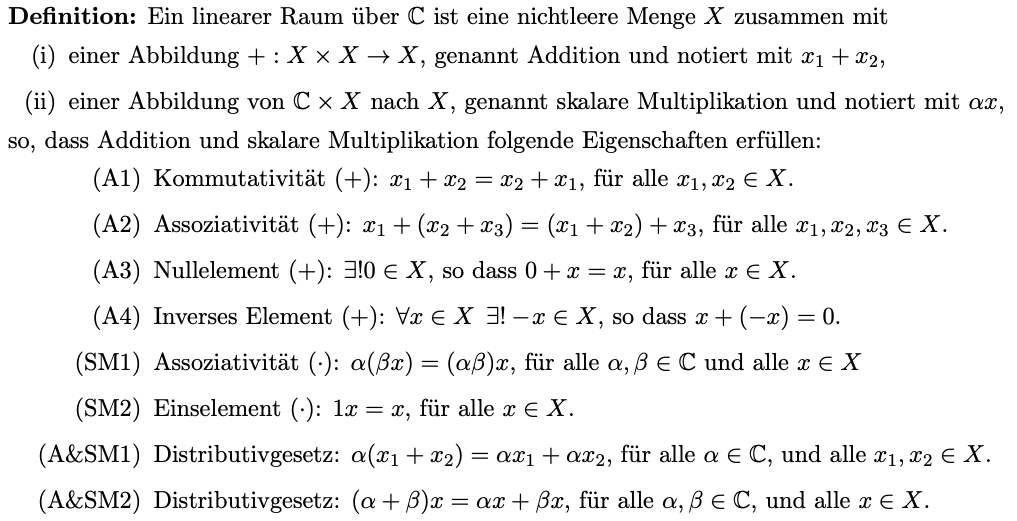
\includegraphics[width=\linewidth]{figures/linearer_raum.png}
\end{frame}

\begin{frame}{Aufgabe 7}
\end{frame}

\begin{frame}{Lineare Unterräume}
    \begin{itemize}
        \item \textbf{Definition:} Ein linearer Unterraum ist eine \textbf{nichtleere Teilmenge} $(\Tilde{X})$ eines linearen Raumes $X$, wenn gilt:
        \item[] 
    \item[] \begin{itemize}
                \item[(i)] $x_1 + x_2 \in \Tilde{X}$, für alle $x_1, x_2 \in \Tilde{X}$.
                \item[] 
                \item[(ii)] $\alpha x \in \Tilde{X}$, für alle $\alpha \in \mathbb{C}$ und alle $x\in \Tilde{X}$.
            \end{itemize}
    \end{itemize}
\end{frame}

\begin{frame}{Aufgabe 9} 
\end{frame}

\begin{frame}{Basen in linearen Räumen}
    \begin{itemize}
    \item[] \textbf{Definition:} Eine Teilmenge $\{ x_i\}_{i=1}^n$ des linearen Raumes $X$ ist linear abhängig, wenn es zugehörige Skalare $\{\alpha_i\}_{i=1}^n$ gibt, die \textbf{nicht alle gleich Null} sind und so, dass $$\sum_{i=1}^n \alpha_i x_i = 0.$$ Wenn $\sum_{i=1}^n \alpha_i x_i = 0$ impliziert, dass $\alpha_i = 0$ für alle $i \in \{ 1, \dots, n\}$, dann ist die Teilmenge $\{ x_i\}_{i=1}^n$ linear unabhängig.
\end{itemize}
\end{frame}

\begin{frame}{Basen in linearen Räumen}
    \begin{itemize}
    \item Die \textbf{Basis} eines linearen Raums $X$ ist eine Menge von Vektoren in $X$, die linear unabhängig sind und jedes Element $x$ des gesamten Raumes $X$ durch eindeutige Linearkombination erzeugen können.
\end{itemize}

\end{frame}

\begin{frame}{Basen in linearen Räumen}
    \begin{itemize}
        \item \textbf{Formale Definition:} Die Menge $\{\mathbf{e}_k\}_{k=1}^M, \; \mathbf{e}_k \in \mathbb{C}^M$, ist eine Basis für $\mathbb{C}^M$, wenn:
    \begin{enumerate}
        \item[] 
        \item $\text{span}\{\mathbf{e}_k\}_{k=1}^M = \mathbb{C}^M$
        \item[] 
        \item $\{\mathbf{e}_k\}_{k=1}^M$ linear unabhängig ist.
    \end{enumerate}
    \end{itemize}
\end{frame}

\begin{frame}{Basen in linearen Räumen}
    \begin{center}
        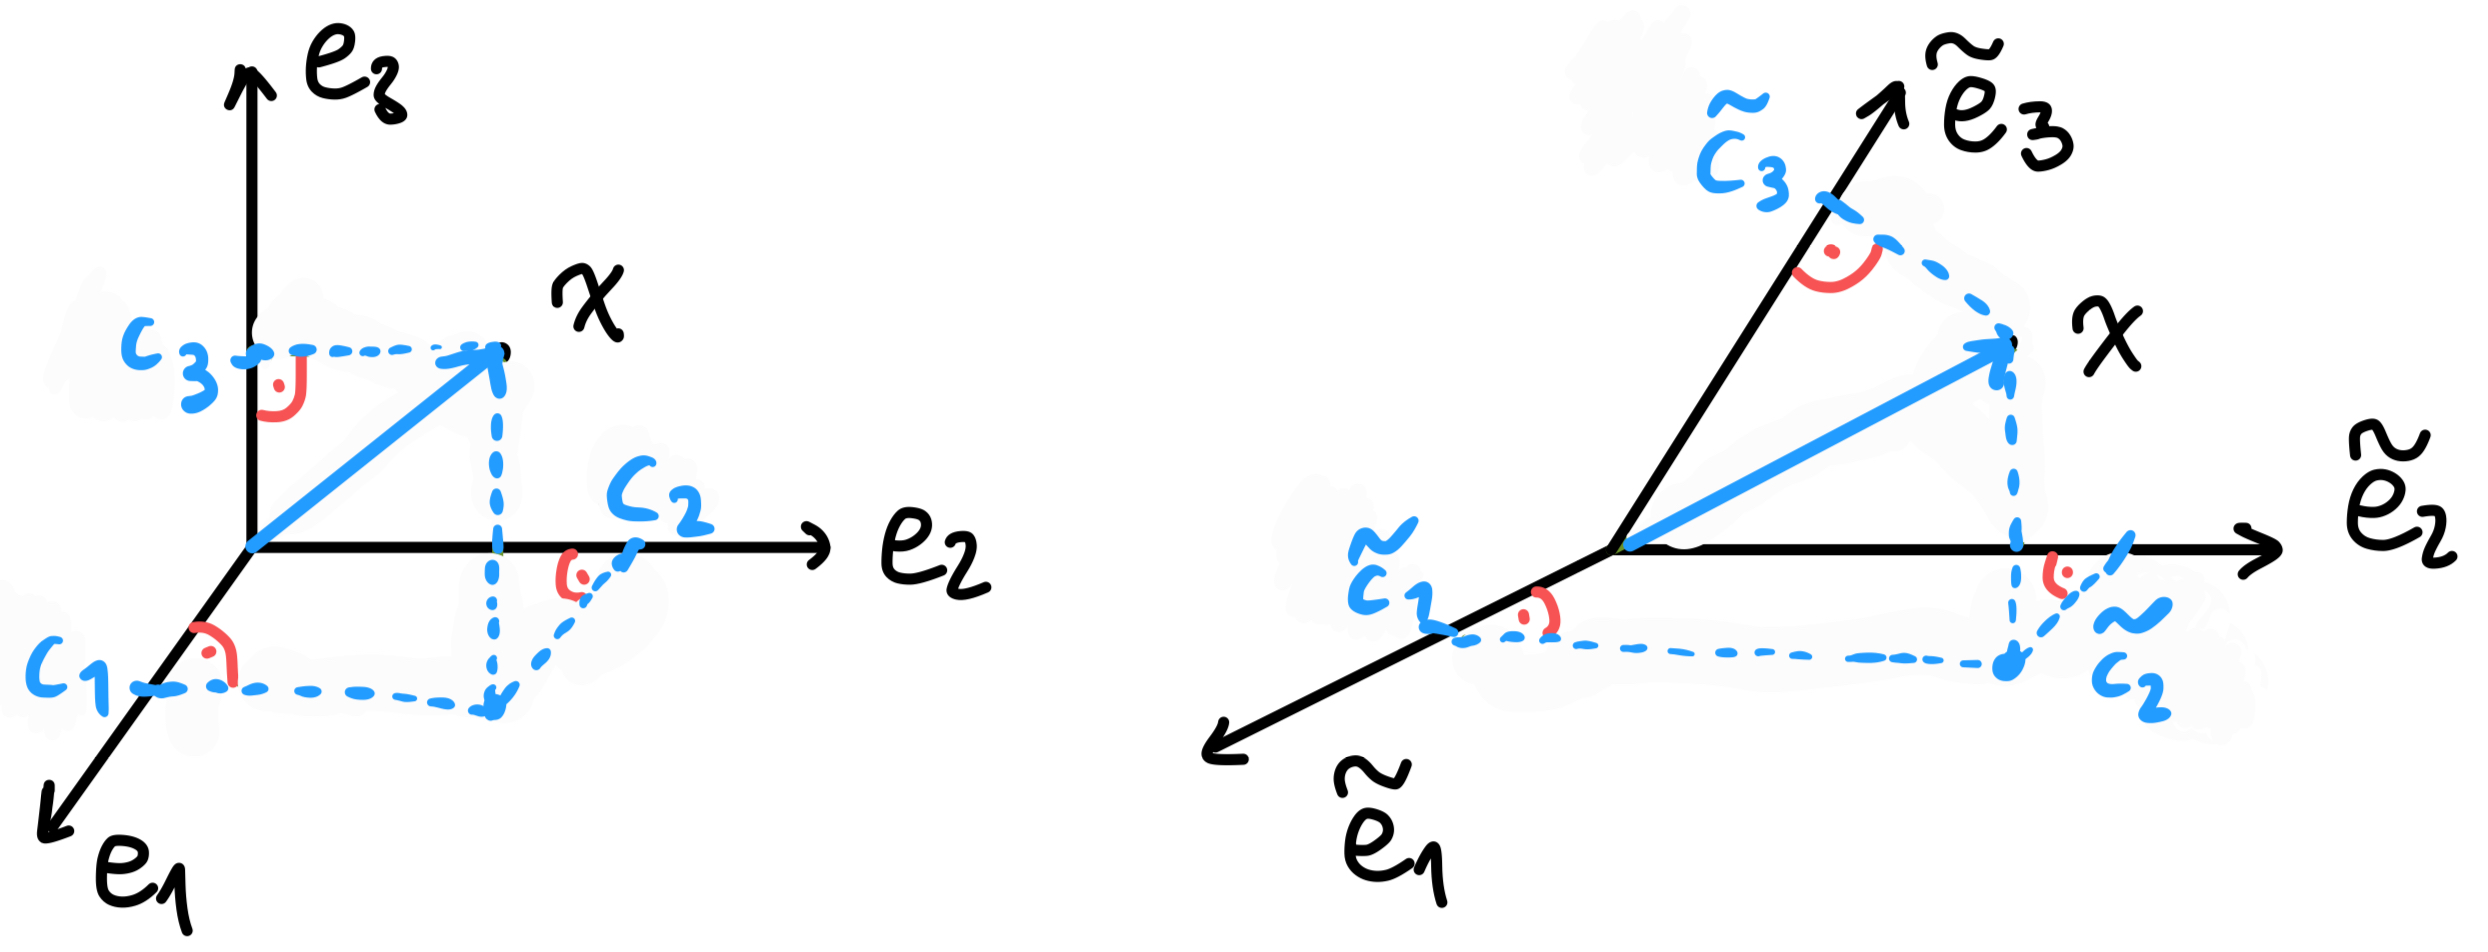
\includegraphics[width=0.6\linewidth]{figures/Basen.jpg}
    \end{center}
    $$\text{Koordinaten } \hspace{5pt} c_k := \langle \mathbf{x}, \; \mathbf{e}_k \rangle, \hspace{10pt} k=1, \dots, M$$
\end{frame}

\begin{frame}{Analysematrix}
    $$\hspace{-6.25cm}\text{Analysematrix } \hspace{5pt} \mathbf{T}:= \begin{bmatrix}
    \mathbf{e}_1^H \\
    \vdots \\
    \mathbf{e}_M^H
\end{bmatrix} $$

$$\text{Koordinaten }\hspace{5pt}  \mathbf{c} = \begin{bmatrix}
    c_1 \\
    \vdots \\
    c_M
\end{bmatrix} = \begin{bmatrix}
    \mathbf{e}_1^H \cdot \mathbf{x}\\
    \vdots \\
    \mathbf{e}_M^H \cdot \mathbf{x}
\end{bmatrix} = \begin{bmatrix}
    \langle \mathbf{e}_1, \; \mathbf{x} \rangle \\
    \vdots \\
    \langle \mathbf{e}_M, \; \mathbf{x} \rangle 
\end{bmatrix} = \mathbf{Tx} \hspace{5pt}$$
\end{frame}

\begin{frame}{Dimensionsbegriff}
    \begin{itemize}
        \item \textbf{Dimension $M$} \begin{itemize}
            \item[$=$] maximale Anzahl linear unabhängiger Elemente im linearen Raum
            \item[] 
            \item[$=$] Anzahl Basiselemente \textbf{jeder} Basis dieses linearen Raumes
        \end{itemize}
        \item[]
        \item Wenn es kein endliches $M$ gibt, $\implies X$ unendlich-dimensional.
    \end{itemize}
\end{frame}

\begin{frame}{Duale Basen}
    \begin{itemize}
        \item Eine Menge $\{\Tilde{\mathbf{e}}_k\}_{k=1}^M, \; \Tilde{\mathbf{e}}_k \in \mathbb{C}^M, \; k = 1,\dots, M$ heisst dual zu einer Basis $\{\mathbf{e}_k\}_{k=1}^M$, wenn:
    $$\mathbf{x} = \sum_{k=1}^M \langle \mathbf{x}, \; \mathbf{e}_k \rangle \Tilde{\mathbf{e}}_k, \hspace{5pt} \text{ für alle } \hspace{5pt} \mathbf{x} \in \mathbb{C}^M$$
    \end{itemize}
\end{frame}

\begin{frame}{Duale Basen einer ONB}
    \begin{itemize}
        \item Die duale Basis einer Orthonormalbasis ist sie selbst. $\Tilde{\mathbf{e}}_k = \mathbf{e}_k, \hspace{5pt} \text{ für alle } k=1, \dots, M$, denn dann gilt trivialerweise:
        \item[] $$\mathbf{x} = \sum_{k=1}^M \langle \mathbf{x}, \; \mathbf{e}_k \rangle \mathbf{e}_k$$
        \item[] 
        \item[] 
        \item[] 
        \item[] 
        \item[] 
        \item[] 
    \end{itemize}
\end{frame}

\begin{frame}{Duale Basen einer allgemeinen Basis}
    \begin{itemize}
        \item \textbf{Synthesematrix:} $\Tilde{\mathbf{T}}^H = \left[\Tilde{\mathbf{e}}_1, \dots,\Tilde{\mathbf{e}}_M \right]$
        \item[] 
        \item Setze $\Tilde{\mathbf{T}}^H = \mathbf{T}^{-1}$, um eine duale Basis zu finden.
        \item[] 
    \end{itemize}
    $$\hspace{-1cm}\implies \Tilde{\mathbf{T}}^H \mathbf{T} \mathbf{x} = \left[\Tilde{\mathbf{e}}_1, \dots,\Tilde{\mathbf{e}}_M \right] \begin{bmatrix}
        \langle \mathbf{x}, \; \mathbf{e}_1 \rangle \\
        \vdots \\
        \langle \mathbf{x}, \; \mathbf{e}_M \rangle
    \end{bmatrix} = \sum_{k=1}^M \langle \mathbf{x}, \; \mathbf{e}_k \rangle \Tilde{\mathbf{e}}_k = \mathbf{x}, \hspace{5pt}$$
\end{frame}

\begin{frame}{Aufgabe 11}
    
\end{frame}

\begin{frame}{Funktionsräume}

\begin{itemize}
    \item Für eine nichtleere Menge $S$ definiert man den linearen Raum $X$ als Menge aller Funktionen von $S$ nach $\mathbb{C}$, wobei die Addition und die skalare Multiplikation wie folgt definiert sind:
    \item[] 
    \item[(+)] $\forall x_1, x_2 \in X \hspace{40pt} +:X \times X \to X \hspace{12pt} $
    \item[] $(x_1 + x_2)(s) = x_1(s) + x_2(s) \hspace{8pt} \forall s \in S$
    \item[] 
    \item[($\cdot$)] $\forall \alpha \in \mathbb{C}, \; x \in X \hspace{20pt} \cdot : \mathbb{C} \times X \to X \hspace{14pt} $
    \item[] $(\alpha \cdot x)(s) = \alpha x(s)$
\end{itemize}
\end{frame}

\begin{frame}{Norm}
\begin{itemize}
    \item \textbf{Definition:} Eine reelle Funktion $||\cdot ||$, definiert auf einem linearen Raum $X$, ist eine Norm auf $X$, wenn gilt:
    \item[] 
    \item[(N1)] Nichtnegativität: $||x|| \geq 0$, für alle $x\in X$
    \item[(N2)] Dreiecksungleichung: $||x_1 + x_2|| \leq ||x_1|| + ||x_2||$, für alle $x_1, x_2\in X$
    \item[(N3)] Homogenität: $||\alpha x|| = |\alpha| ||x||$, für alle $x\in X$
    \item[(N4)] Definitheit: $||x||=0$ dann, und nur dann, wenn $x=0$

\end{itemize}
\end{frame}

\begin{frame}{Normierte Lineare Räume}
    \begin{itemize}
        \item \textbf{Definition:} Ein normierter linearer Raum ist ein Paar $(X, ||\cdot||)$ bestehend aus einem linearen Raum $X$ und einer Norm auf $X$.
    \end{itemize}
\end{frame}

\begin{frame}{Beispiele für Normierte Lineare Räume}
    \begin{itemize}
        \item linearer Raum $\mathbb{R}^n$ oder $\mathbb{C}^n$ mit einer der folgenden Normen: \begin{itemize}
        \item[] 
        \item[] Summennorm (1-Norm): $\hspace{22pt}||\mathbf{x}||_1 = \sum_{i=1}^n |x_i|$
        \item[] 
        \item[] Euklidische Norm (2-Norm): $\hspace{3pt}||\mathbf{x}||_2 = \sqrt{\sum_{i=1}^n |x_i|^2}$
        \item[] 
        \item[] p-Norm: $\hspace{100pt}||\mathbf{x}||_p = \left(\sum_{i=1}^n |x_i|^p\right)^{1/p}$ für $1\leq p < \infty$
        \item[] 
        \item[] Maximumsnorm: $\hspace{60pt}||\mathbf{x}||_\infty = \underset{i=1,\dots,n}{\max}|x_i|$
        \end{itemize}
    \end{itemize}
\end{frame}

\begin{frame}{Beispiele für Normierte Lineare Räume}
    \begin{itemize}
        \item linearer Raum $L^p := \{ x:\mathbb{R}\to \mathbb{C} : \int_{-\infty}^\infty |x(t)|^p \text{dt} < \infty \} $ \\mit der Norm $||x||_{L^p} := \left( \int_{-\infty}^\infty |x(t)|^p \text{dt}\right)^{1/p}$
        \item[] 
        \item linearer Raum $l^p :=\{ x:\mathbb{Z}\to \mathbb{C} : \sum_{n=-\infty}^\infty |x[n]|^p < \infty \} $ \\mit der Norm $||x||_{l^p} := \left( \sum_{n=-\infty}^\infty |x[n]|^p \right)^{1/p}$
    \end{itemize}
\end{frame}

\begin{frame}{Einteilung der Signale}
    \begin{center}
            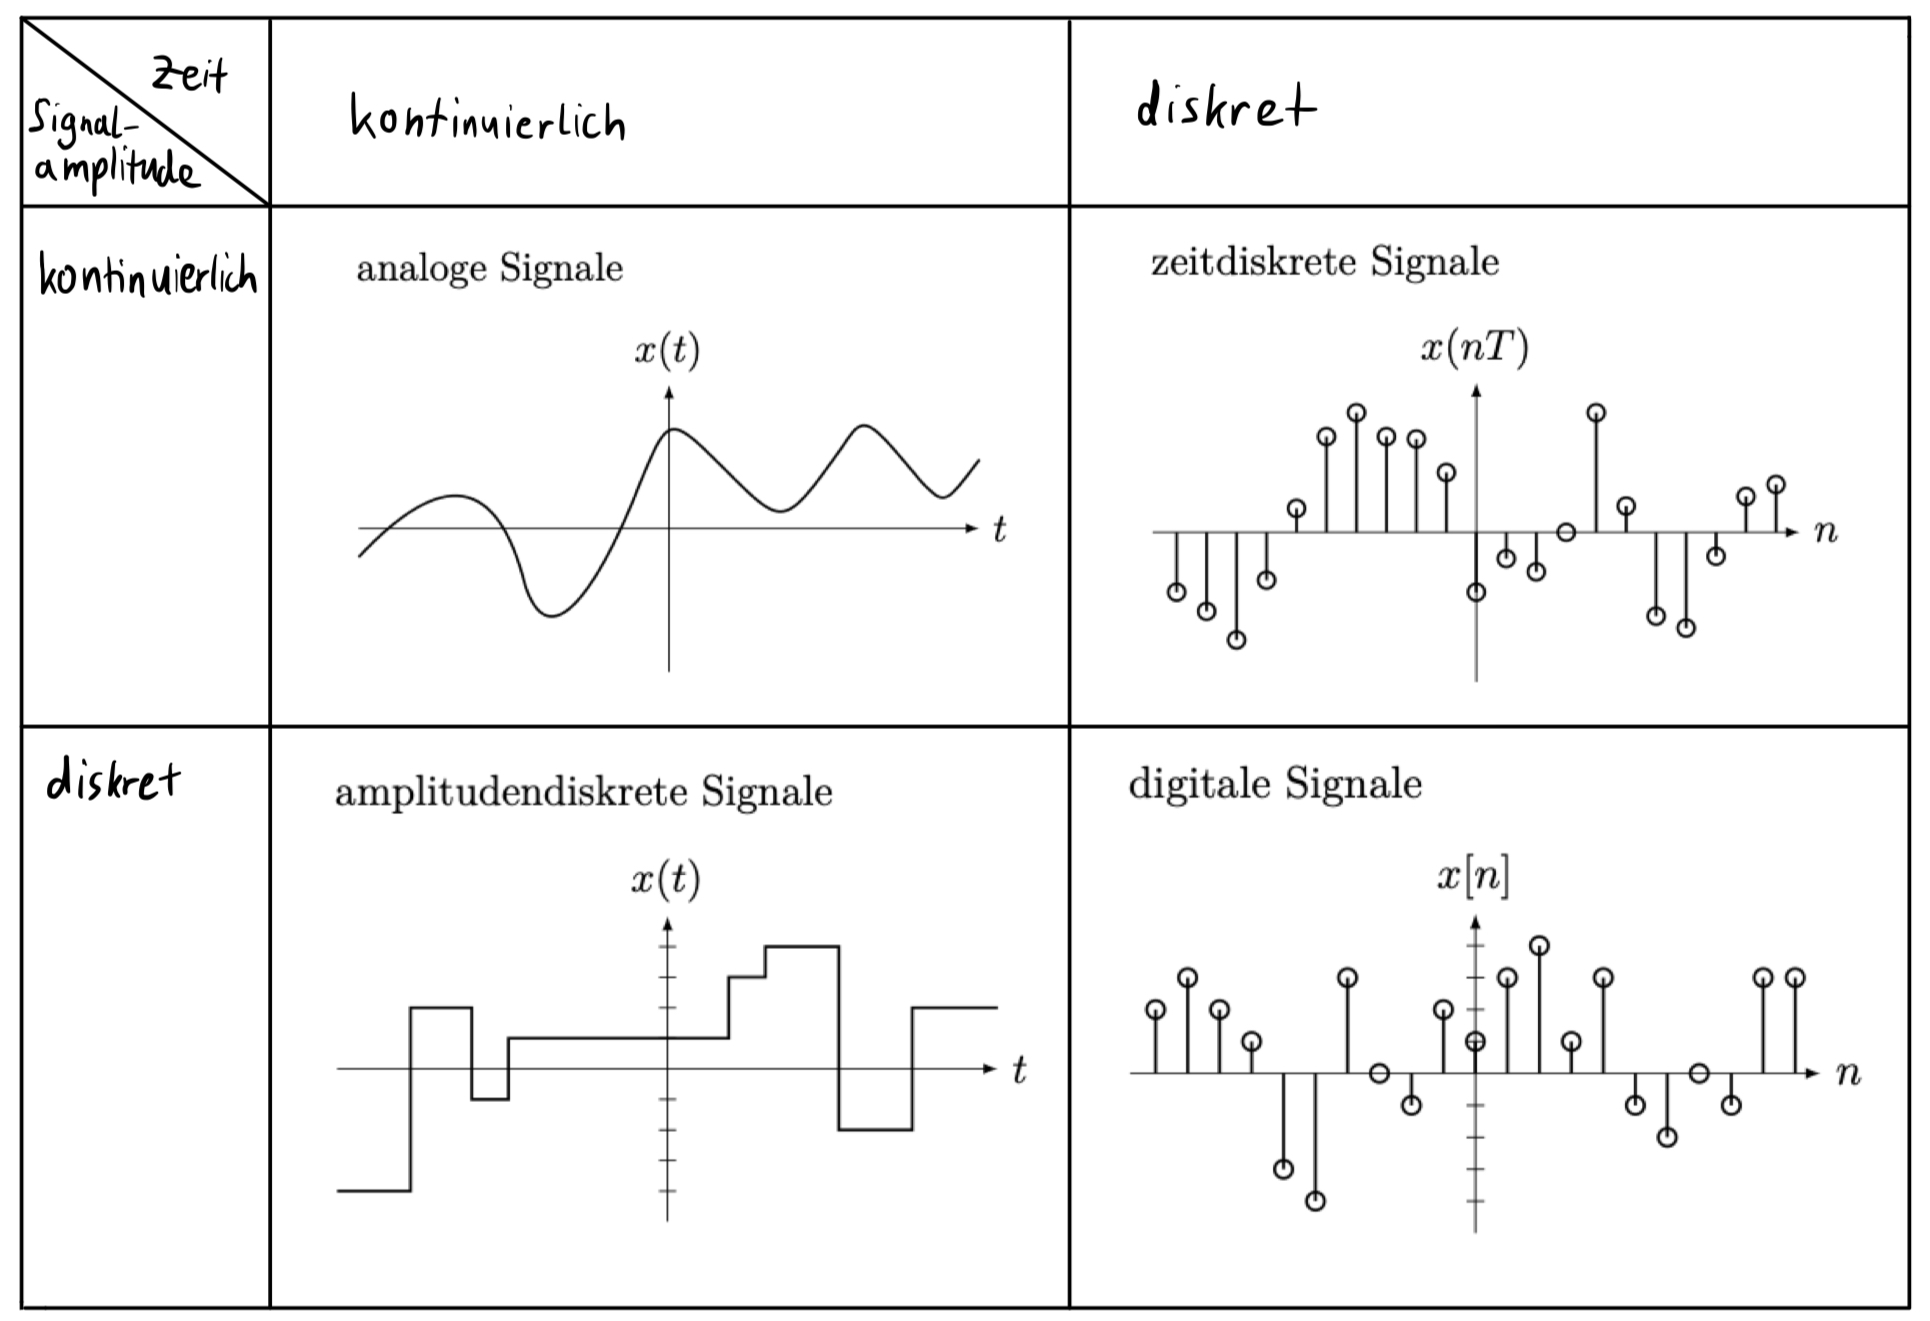
\includegraphics[width=0.7\linewidth]{figures/Signale.jpg}
    \end{center}
\end{frame}


\end{document}
